%\UseRawInputEncoding
\documentclass[a4paper,10pt]{article}
\usepackage[utf8]{inputenc}
\usepackage{amsmath}
\usepackage{fullpage}
\usepackage{hyperref}
\usepackage{graphicx}
\usepackage{listings}
\usepackage{color}

\definecolor{mygreen}{rgb}{0,0.6,0}
\definecolor{mygray}{rgb}{0.5,0.5,0.5}
\definecolor{mymauve}{rgb}{0.58,0,0.82}

\lstset{ 
  backgroundcolor=\color{white},   % choose the background color; you must add \usepackage{color} or \usepackage{xcolor}; should come as last argument
  basicstyle=\footnotesize,        % the size of the fonts that are used for the code
  breakatwhitespace=false,         % sets if automatic breaks should only happen at whitespace
  breaklines=true,                 % sets automatic line breaking
  captionpos=b,                    % sets the caption-position to bottom
  commentstyle=\color{mygreen},    % comment style
  deletekeywords={...},            % if you want to delete keywords from the given language
  escapeinside={\%*}{*)},          % if you want to add LaTeX within your code
  extendedchars=true,              % lets you use non-ASCII characters; for 8-bits encodings only, does not work with UTF-8
  firstnumber=1,                   % start line enumeration with line 1000
  frame=single,	                   % adds a frame around the code
  keepspaces=true,                 % keeps spaces in text, useful for keeping indentation of code (possibly needs columns=flexible)
  keywordstyle=\color{blue},       % keyword style
  language=Python,                 % the language of the code
  morekeywords={*,...},            % if you want to add more keywords to the set
  numbers=left,                    % where to put the line-numbers; possible values are (none, left, right)
  numbersep=5pt,                   % how far the line-numbers are from the code
  numberstyle=\tiny\color{mygray}, % the style that is used for the line-numbers
  rulecolor=\color{black},         % if not set, the frame-color may be changed on line-breaks within not-black text (e.g. comments (green here))
  showspaces=false,                % show spaces everywhere adding particular underscores; it overrides 'showstringspaces'
  showstringspaces=false,          % underline spaces within strings only
  showtabs=false,                  % show tabs within strings adding particular underscores
  stepnumber=1,                    % the step between two line-numbers. If it's 1, each line will be numbered
  stringstyle=\color{mymauve},     % string literal style
  tabsize=4,	                   % sets default tabsize to 2 spaces
  title=\lstname                   % show the filename of files included with \lstinputlisting; also try caption instead of title
}


%opening
\title{NUR - Hand-in Exercise 1}
\author{Martina Cacciola}

\begin{document}

\maketitle

\begin{abstract}
 In this document an example solution template is given for the exercises in the 
 course Numerical recipes for astrophysics.
\end{abstract}

%\section{Ex. 1 - 2. Vandermonde matrix}
%\lstinputlisting{vandermonde.py}

In this section, we add the comments to the plots produced by the script given by: vandermonde.py.
For question (a), we are performing a polynomial interpolation on a set of data points using a 19th-degree polynomial, evaluated at $\approx$ 1000 equally-spaced points. The coefficients of the polynomial are determined by solving a system of linear equations using LU decomposition. We also plot the absolute difference between the given points $y_{i}$ and our result $y(x)$, i.e. $|y(x) - y_{i}|$. \\

From Fig.\ref{fig:lu_dec}, it seems that the polynomial is fitting the data points quite well for most of the range. This is expected as a polynomial of degree ($n$) can always fit ($n+1$) data points exactly. However, towards the end (around $x=100$), the polynomial shoots up drastically. This is a common issue with high-degree polynomial interpolation known as Runge's phenomenon. It is a form of overfitting where the polynomial oscillates significantly at the boundaries of the data set.

The choice of a 19th-degree polynomial for this data might not be the best. While it fits the given data points well, the extreme behavior at the boundaries suggests that it might not generalize well to other data. A lower-degree polynomial or a different type of function might provide a better fit without the extreme oscillations. \\

The bottom part of the plot shows the absolute difference between the given $y_{i}$ values and the calculated $y(x)$ values. This represents the error in the polynomial fit at the data points. Since the polynomial fits the data points exactly, these errors are close to zero, going from order $10^{-14}$ to $10^{-2}$. We can note how the error increases at the boundaries, consistently with the issue presented before. \\

For question (b), we implement Neville's algorithm and compare it to the results from LU decomposition (see Fig. \ref{fig:neville}).It works by recursively evaluating a set of polynomials and combining them to form the final interpolating polynomial. Regarding the interpolation, we are getting the same results, so they have same efficiency in fitting the given data points. The errors are drastically small for Neville's (reaching a maximum of $10^{-14}$) while LU decomposition have errors slightly higher. We could explain this addressing to the nature of the algorithm, which tends to be stable and accurate, especially when the data points are equally spaced. The accuracy of LU decomposition for interpolation can be influenced by the condition of the matrix involved. Ill-conditioned matrices may lead to numerical instability and higher errors. In our case, the condition number of the Vandermonde matrix depends on the arrangement and spacing of the data points. If the data points are well-spaced and not too close to each other, the condition number may be reasonable. However, as the data points become closely spaced or nearly collinear, the problem of ill-conditioning can arise. \\

For question (c), we improve iteratively the solution found by LU decomposition. We do such procedure for 1 and 10 iterations (Fig. \ref{fig:lu_iter}).
The interpolation is the same for both cases, since we have overlapping fits also in this case. Regarding the trend for the error, the two procedures get similar results, with the LU having a slightly lower errors in some regions of the data.

For question (d), we obtain the execution times for LU decomposition, Neville's algorithm, and LU with iterative improvement. 
\begin{itemize}
    \item \textbf{LU Decomposition Time}: 0.012404 seconds. The algorithm is known for its efficiency in solving linear systems of equations, and it typically has a low time complexity. This outcome indicates that LU decomposition is well-suited for our data set.

    \item \textbf{Neville's Algorithm Time}: 9.874374 seconds. The algorithm involves several polynomial evaluations and recursive calculations: the complexity of these calculations can lead to longer execution times, especially as the number of data points increases.
    
    \item \textbf{Iterative Improvement Time}: 0.117441 seconds. It is refining a solution through iterative steps, in a relatively fast process. The efficiency of this process can depend on the convergence behavior of the iterative method and the initial guess.
    
\end{itemize}
 
From these results, the LU decomposition method appears to be the most efficient in terms of computational time. If we take the speed as a critical factor and the accuracy achieved by LU decomposition is sufficient for your application, then LU decomposition may be the preferred choice. In our case, the accuracy achieved by LU decomposition is sufficient for our application. However, we have to keep in mind that LU decomposition, while efficient, might be sensitive to ill-conditioned matrices, potentially affecting accuracy in certain cases. In general, accuracy depends on the interpolation requirements and the nature of your data. However, Neville's algorithm is generally considered accurate, especially for well-behaved, evenly spaced data. In our implementation, it is behaving considerably slower than the other, so it might not be the suitable option for this particular setting, even though it is reaching the best performance in terms of lowest errors in the interpolation.


\begin{figure}[h!]
  \centering
  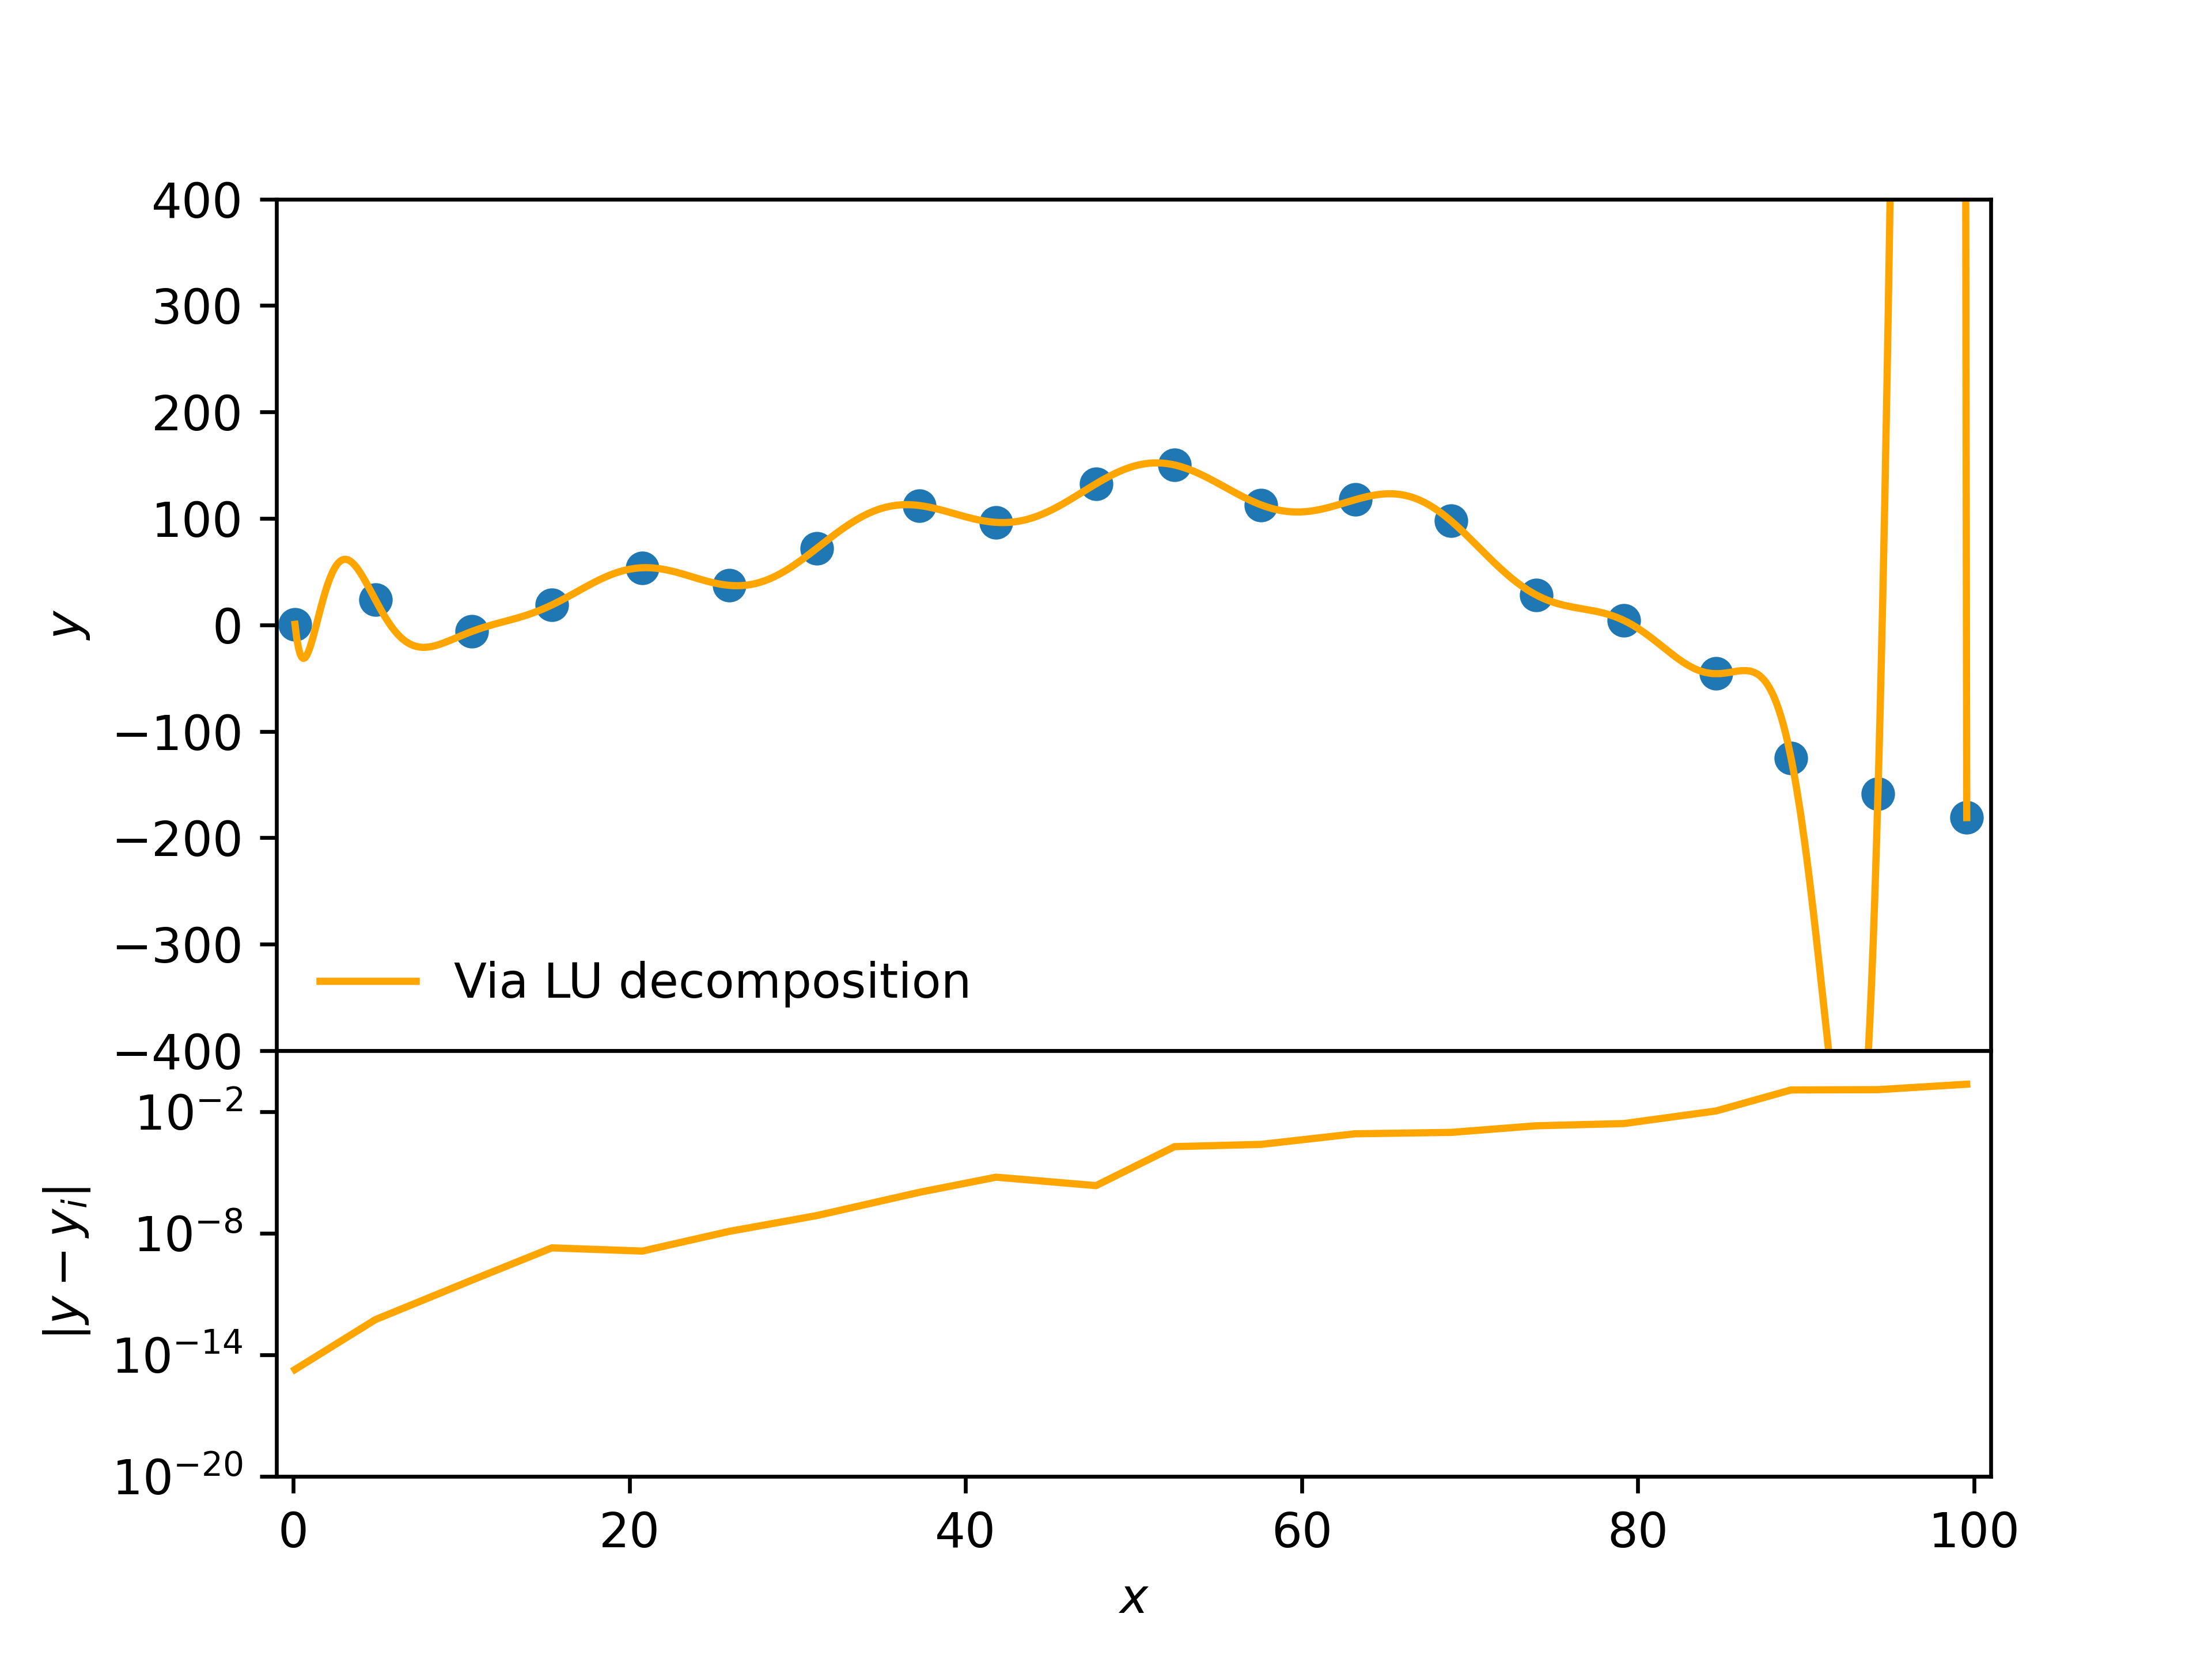
\includegraphics[width=0.9\linewidth]{plots/my_vandermonde_sol_2a.png}
  \caption{Upper panel: Interpolation on a set of given data points via LU decomposition and Neville's. The fit is going through all the data points exactly. Nevertheless, it has an oscillating behaviour in correspondence of the last two points. Bottom panel: Absolute difference between the given points $y_i$ and our result $y(x)$, i.e. $|y(x) − y_{i}|$. The error holds at values close to zero, with a small increase towards the boundaries.}
  \label{fig:lu_dec}
\end{figure}

\begin{figure}[h!]
  \centering
  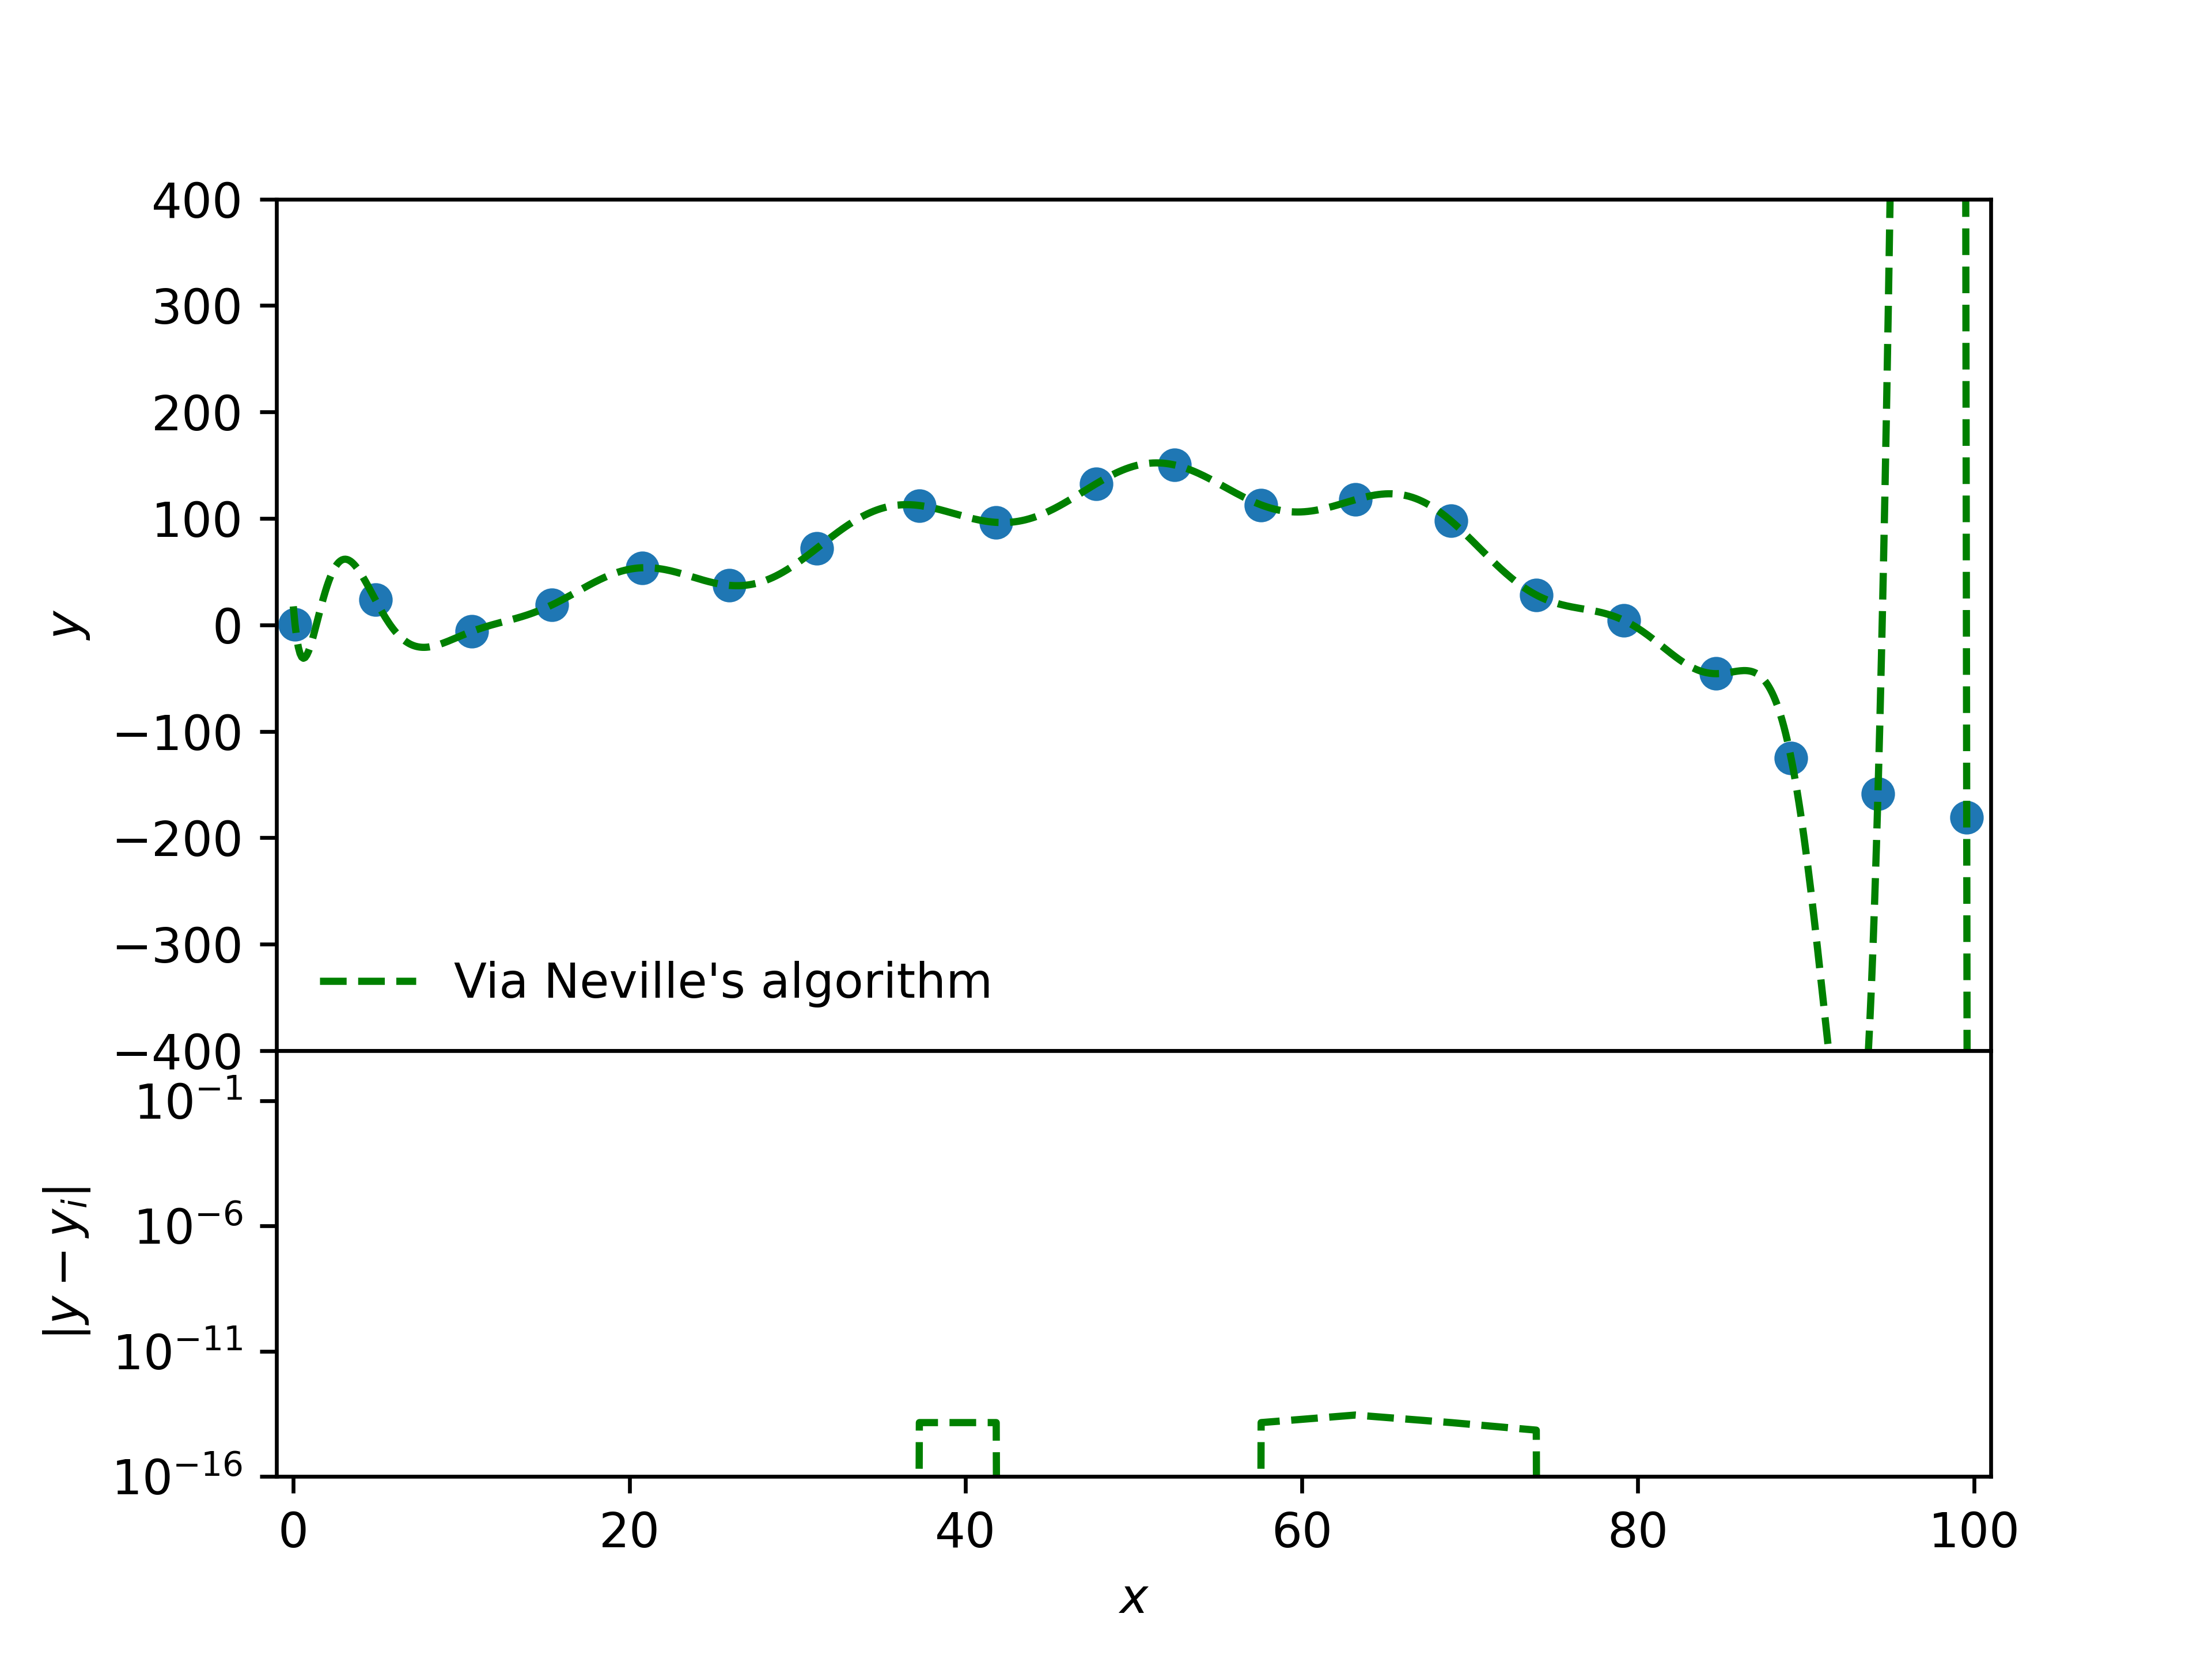
\includegraphics[width=0.9\linewidth]{plots/my_vandermonde_sol_2b.png}
  \caption{Upper panel: Interpolation on a set of given data points via LU decomposition and Neville's algorithm. Both the polynomials obtained fits the data points well in the range considered, confirmed by their interpolations overlapping. Bottom panel: Absolute difference between the given points $y_i$ and our result $y(x)$, i.e. $|y(x) − y_{i}|$. The errors of Neville's algorithm reach very small values with respect to LU decomposition's ones. }
  \label{fig:neville}
\end{figure}

\begin{figure}[h!]
  \centering
  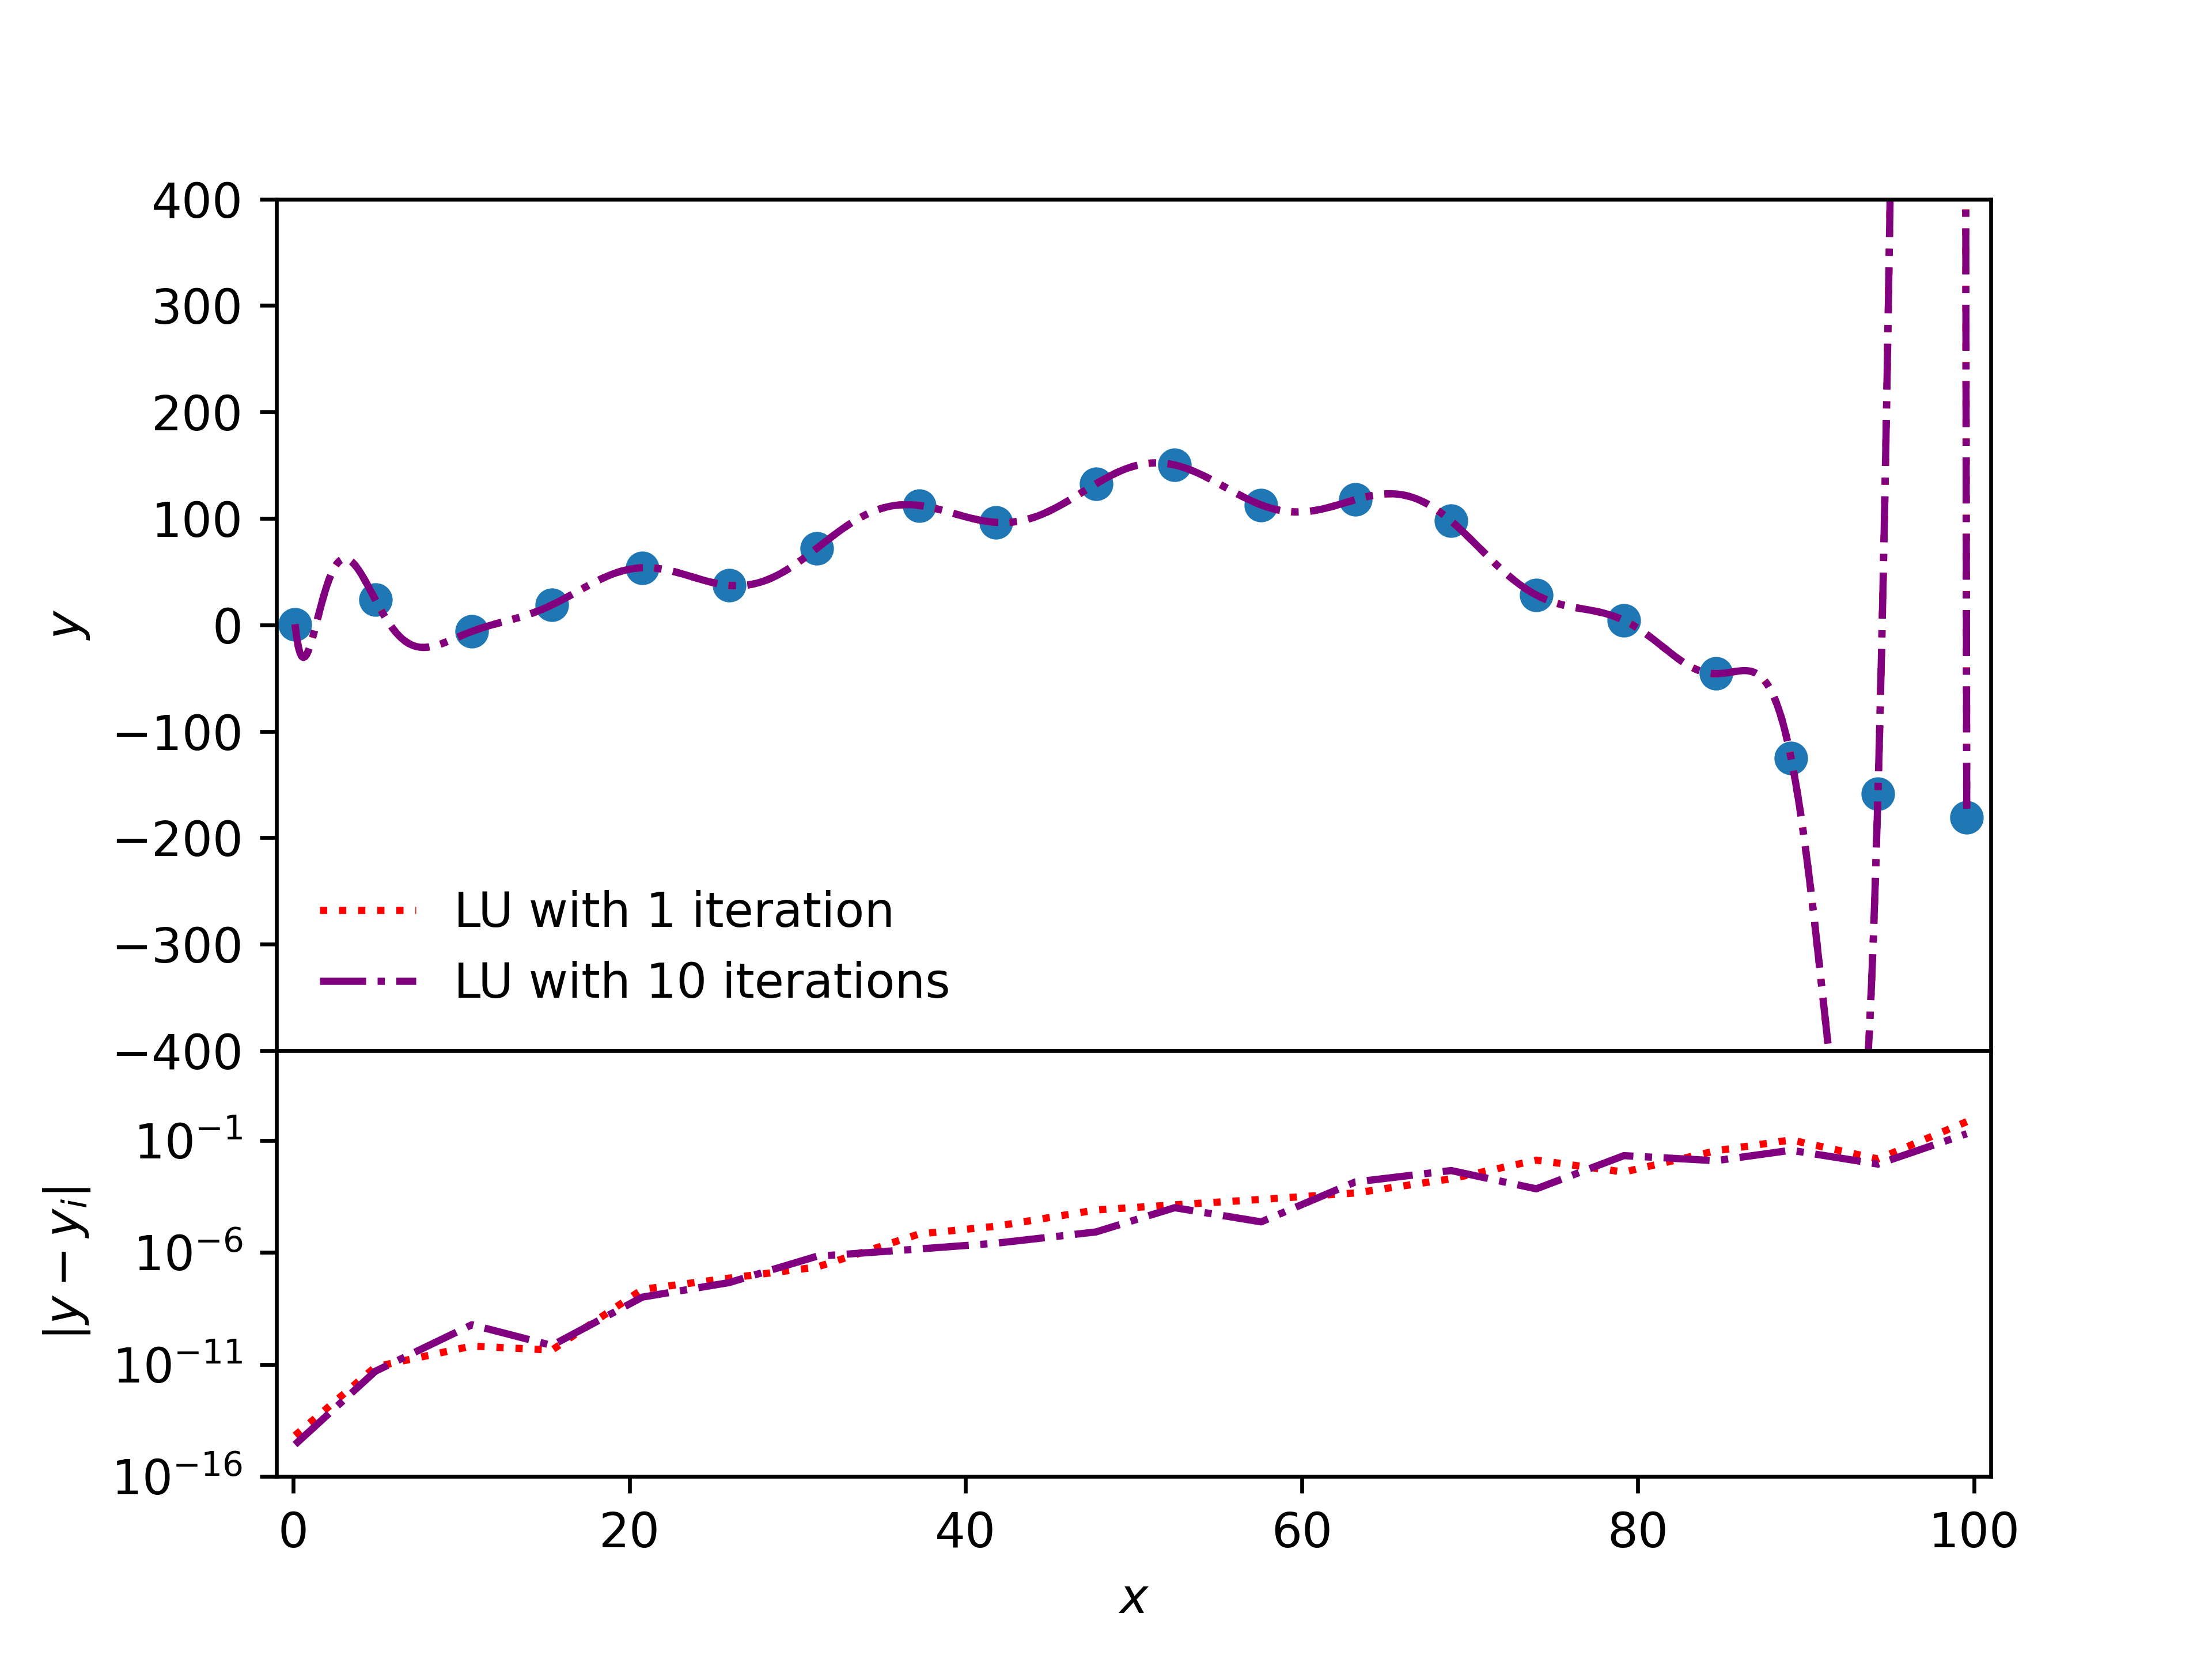
\includegraphics[width=0.9\linewidth]{plots/my_vandermonde_sol_2c.png}
  \caption{Upper panel: Interpolation on a set of given data points via LU decomposition and Neville's. The fit is going through all the data points exactly. Nevertheless, it has an oscillating behaviour in correspondence of the last two points. Bottom panel: Absolute difference between the given points $y_i$ and our result $y(x)$, i.e. $|y(x) − y_{i}|$. The error holds at values close to zero, with a small increase towards the boundaries.}
  \label{fig:lu_iter}
\end{figure}

\section{Vandermonde matrix}
%\lstinputlisting{vandermonde.py}

In this section, we add the comments to the plots produced by the script given by: vandermonde.py.
For question (a), we are performing a polynomial interpolation on a set of data points using a 19th-degree polynomial, evaluated at $\approx$ 1000 equally-spaced points. The coefficients of the polynomial are determined by solving a system of linear equations using LU decomposition. We also plot the absolute difference between the given points $y_{i}$ and our result $y(x)$, i.e. $|y(x) - y_{i}|$. \\

From Fig.\ref{fig:lu_dec}, it seems that the polynomial is fitting the data points quite well for most of the range. This is expected as a polynomial of degree ($n$) can always fit ($n+1$) data points exactly. However, towards the end (around $x=100$), the polynomial shoots up drastically. This is a common issue with high-degree polynomial interpolation known as Runge's phenomenon. It is a form of overfitting where the polynomial oscillates significantly at the boundaries of the data set.

The choice of a 19th-degree polynomial for this data might not be the best. While it fits the given data points well, the extreme behavior at the boundaries suggests that it might not generalize well to other data. A lower-degree polynomial or a different type of function might provide a better fit without the extreme oscillations. \\

The bottom part of the plot shows the absolute difference between the given $y_{i}$ values and the calculated $y(x)$ values. This represents the error in the polynomial fit at the data points. Since the polynomial fits the data points exactly, these errors are close to zero, going from order $10^{-14}$ to $10^{-2}$. We can note how the error increases at the boundaries, consistently with the issue presented before. \\

For question (b), we implement Neville's algorithm and compare it to the results from LU decomposition (see Fig. \ref{fig:neville}).It works by recursively evaluating a set of polynomials and combining them to form the final interpolating polynomial. Regarding the interpolation, we are getting the same results, so they have same efficiency in fitting the given data points. The errors are drastically small for Neville's (reaching a maximum of $10^{-14}$) while LU decomposition have errors slightly higher. We could explain this addressing to the nature of the algorithm, which tends to be stable and accurate, especially when the data points are equally spaced. The accuracy of LU decomposition for interpolation can be influenced by the condition of the matrix involved. Ill-conditioned matrices may lead to numerical instability and higher errors. In our case, the condition number of the Vandermonde matrix depends on the arrangement and spacing of the data points. If the data points are well-spaced and not too close to each other, the condition number may be reasonable. However, as the data points become closely spaced or nearly collinear, the problem of ill-conditioning can arise. \\

For question (c), we improve iteratively the solution found by LU decomposition. We do such procedure for 1 and 10 iterations (Fig. \ref{fig:lu_iter}).
The interpolation is the same for both cases, since we have overlapping fits also in this case. Regarding the trend for the error, the two procedures get similar results, with the LU having a slightly lower errors in some regions of the data.

For question (d), we obtain the execution times for LU decomposition, Neville's algorithm, and LU with iterative improvement. 
\begin{itemize}
    \item \textbf{LU Decomposition Time}: 0.012404 seconds. The algorithm is known for its efficiency in solving linear systems of equations, and it typically has a low time complexity. This outcome indicates that LU decomposition is well-suited for our data set.

    \item \textbf{Neville's Algorithm Time}: 9.874374 seconds. The algorithm involves several polynomial evaluations and recursive calculations: the complexity of these calculations can lead to longer execution times, especially as the number of data points increases.
    
    \item \textbf{Iterative Improvement Time}: 0.117441 seconds. It is refining a solution through iterative steps, in a relatively fast process. The efficiency of this process can depend on the convergence behavior of the iterative method and the initial guess.
    
\end{itemize}
 
From these results, the LU decomposition method appears to be the most efficient in terms of computational time. If we take the speed as a critical factor and the accuracy achieved by LU decomposition is sufficient for your application, then LU decomposition may be the preferred choice. In our case, the accuracy achieved by LU decomposition is sufficient for our application. However, we have to keep in mind that LU decomposition, while efficient, might be sensitive to ill-conditioned matrices, potentially affecting accuracy in certain cases. In general, accuracy depends on the interpolation requirements and the nature of your data. However, Neville's algorithm is generally considered accurate, especially for well-behaved, evenly spaced data. In our implementation, it is behaving considerably slower than the other, so it might not be the suitable option for this particular setting, even though it is reaching the best performance in terms of lowest errors in the interpolation.


\begin{figure}[h!]
  \centering
  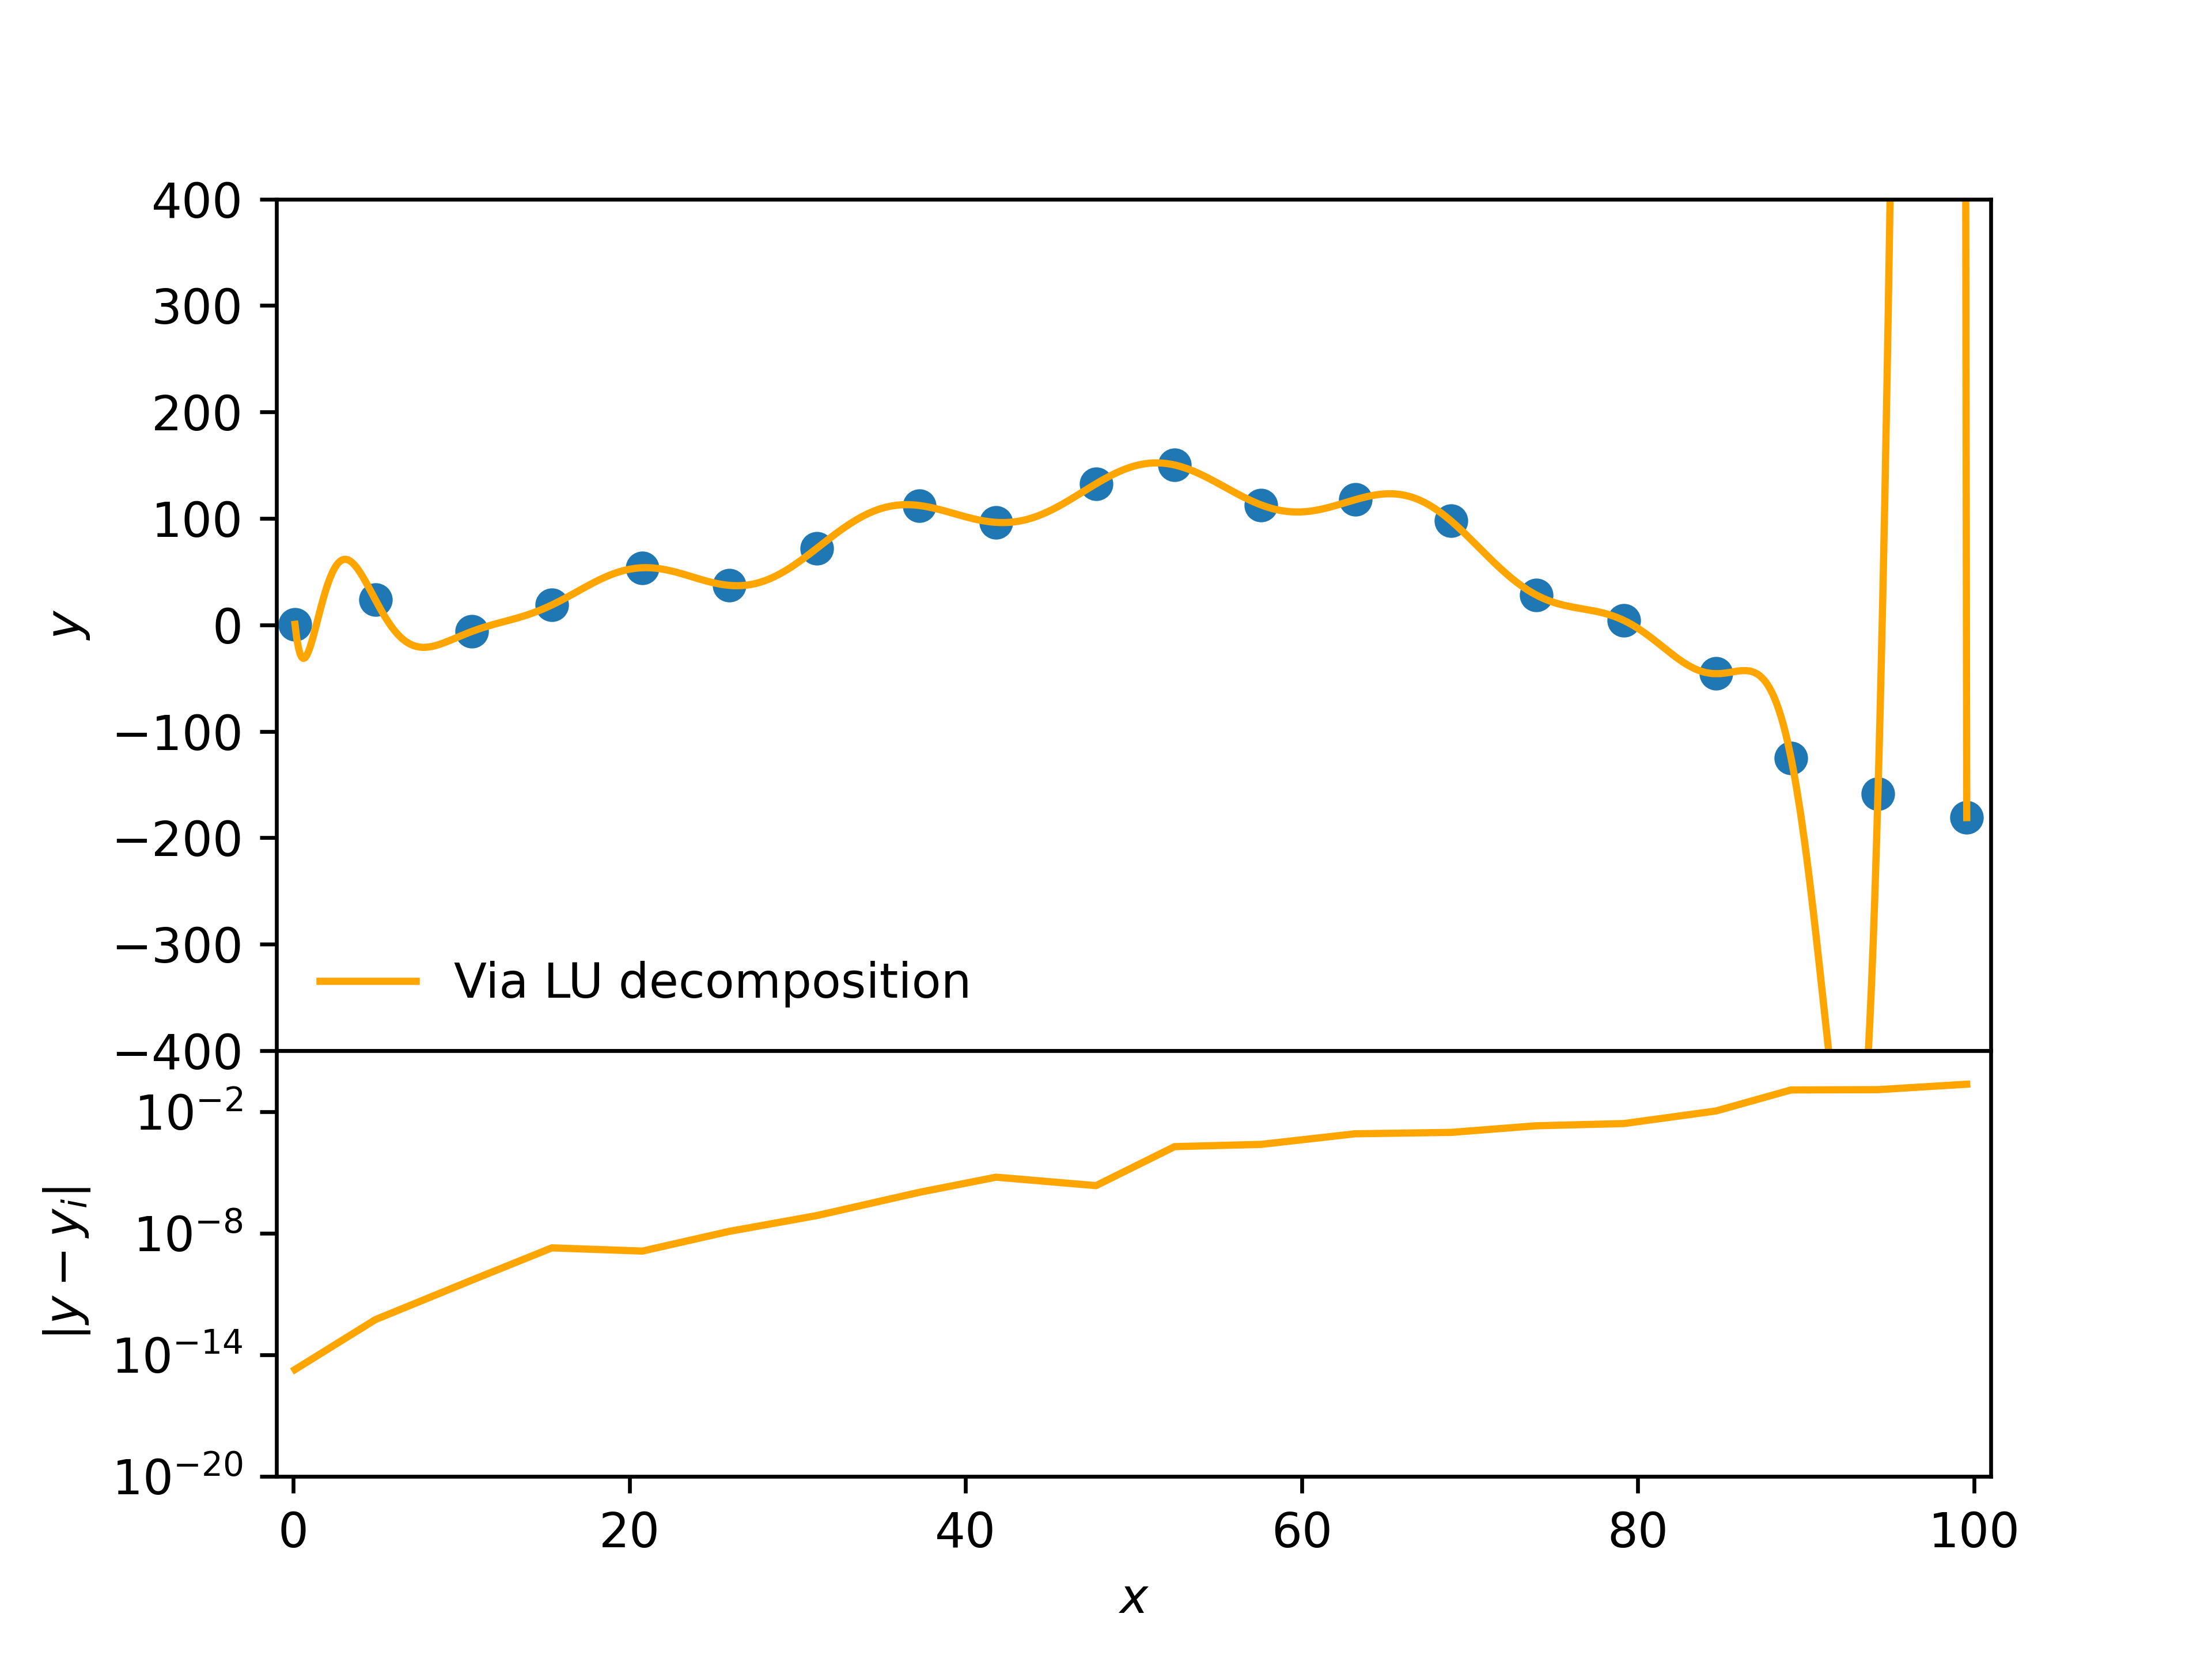
\includegraphics[width=0.9\linewidth]{./plots/my_vandermonde_sol_2a.png}
  \caption{Upper panel: Interpolation on a set of given data points via LU decomposition and Neville's. The fit is going through all the data points exactly. Nevertheless, it has an oscillating behaviour in correspondence of the last two points. Bottom panel: Absolute difference between the given points $y_i$ and our result $y(x)$, i.e. $|y(x) - y_{i}|$. The error holds at values close to zero, with a small increase towards the boundaries.}
  \label{fig:lu_dec}
\end{figure}

\begin{figure}[h!]
  \centering
  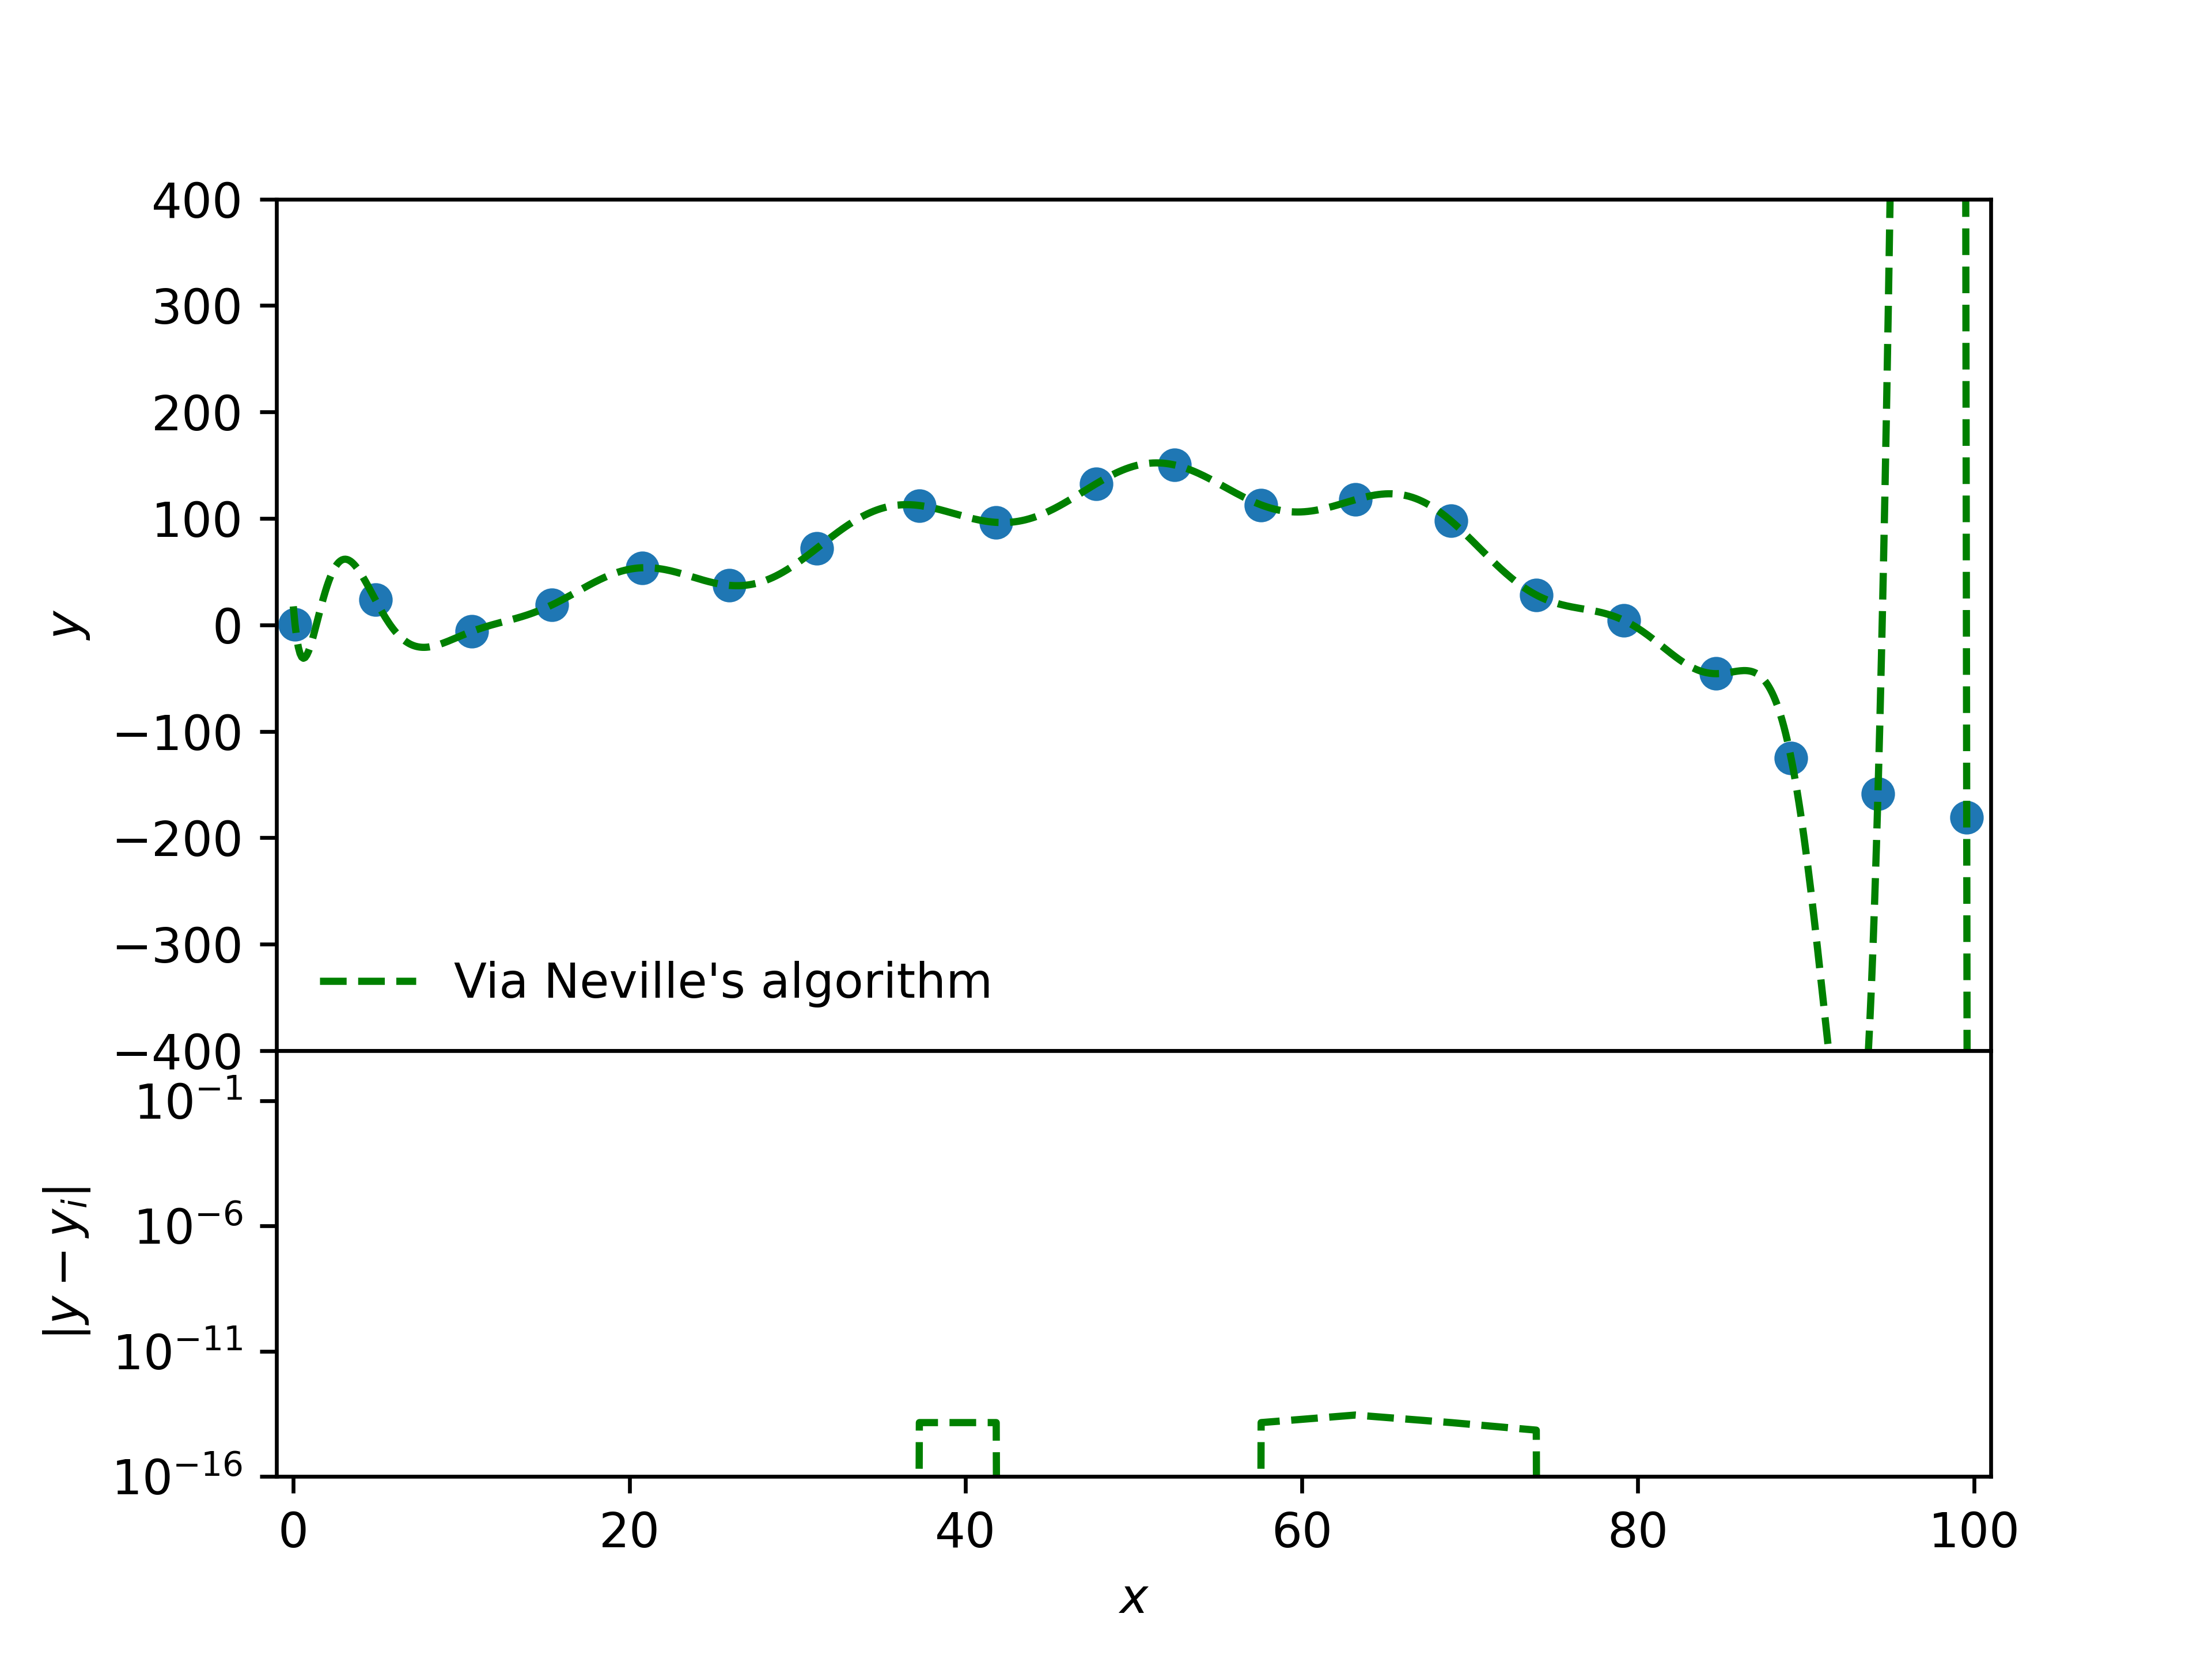
\includegraphics[width=0.9\linewidth]{./plots/my_vandermonde_sol_2b.png}
  \caption{Upper panel: Interpolation on a set of given data points via LU decomposition and Neville's algorithm. Both the polynomials obtained fits the data points well in the range considered, confirmed by their interpolations overlapping. Bottom panel: Absolute difference between the given points $y_i$ and our result $y(x)$, i.e. $|y(x) - y_{i}|$. The errors of Neville's algorithm reach very small values with respect to LU decomposition's ones. }
  \label{fig:neville}
\end{figure}

\begin{figure}[h!]
  \centering
  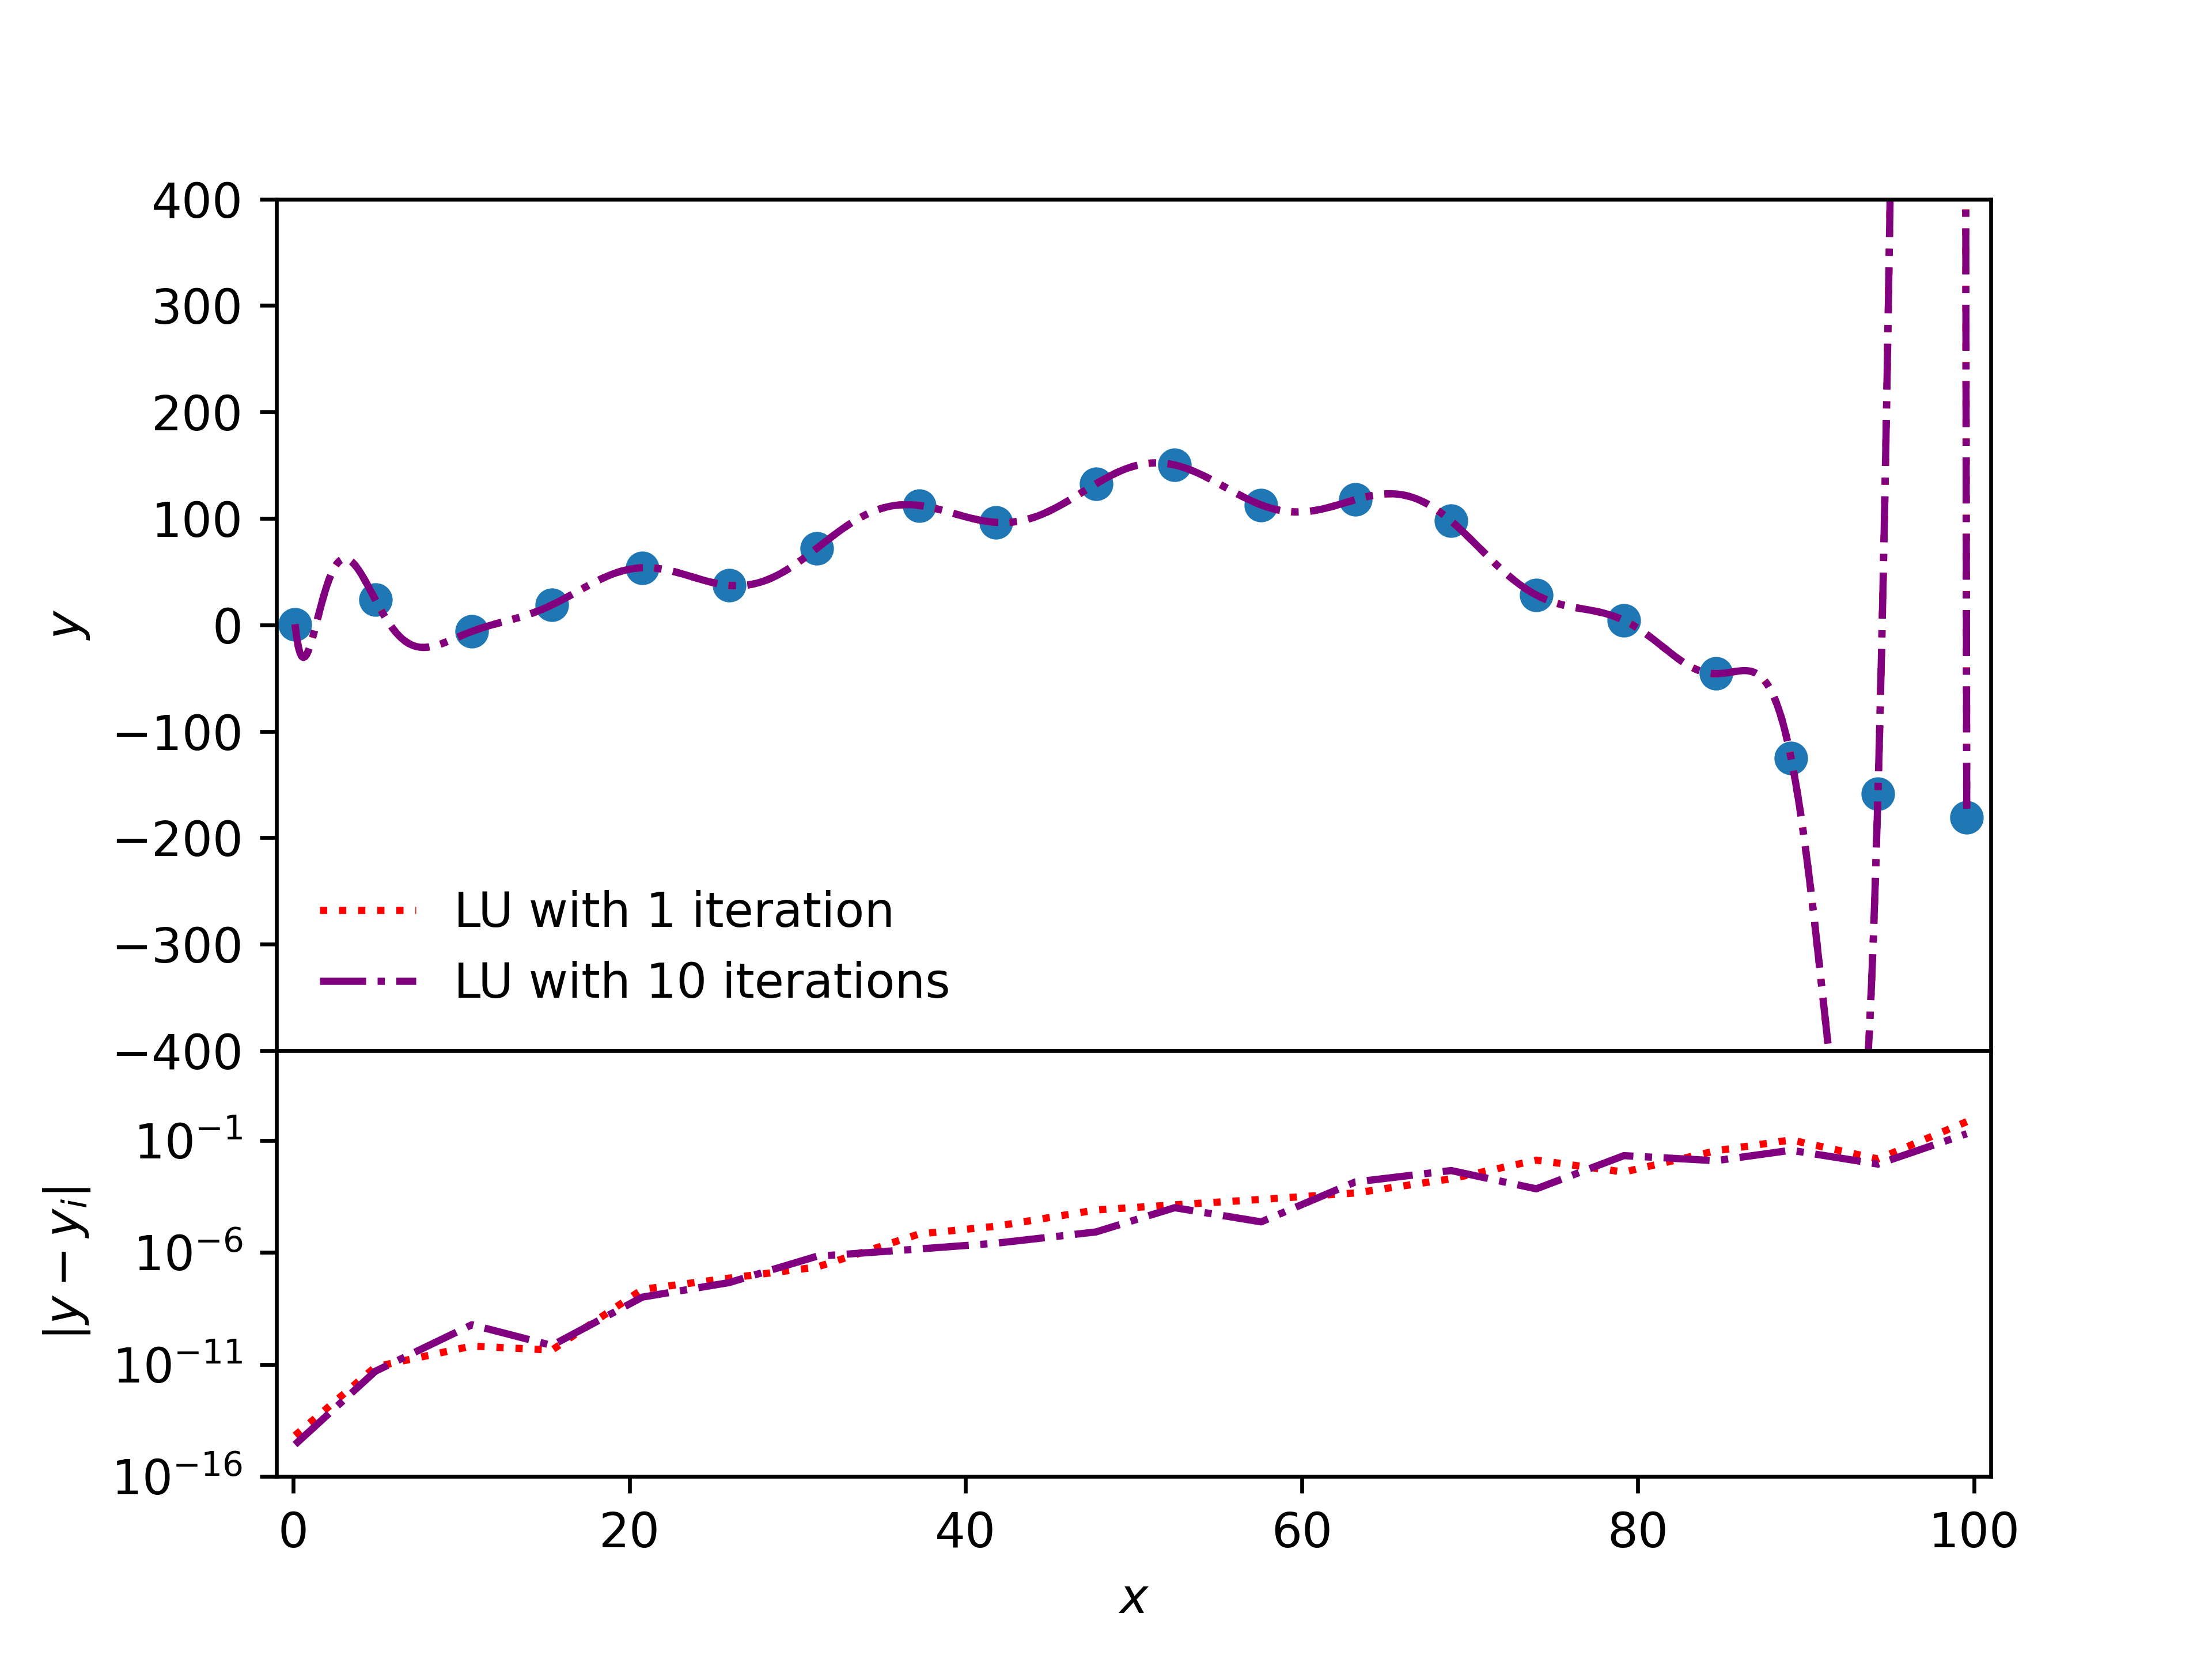
\includegraphics[width=0.9\linewidth]{./plots/my_vandermonde_sol_2c.png}
  \caption{Upper panel: Interpolation on a set of given data points via LU decomposition and Neville's. The fit is going through all the data points exactly. Nevertheless, it has an oscillating behaviour in correspondence of the last two points. Bottom panel: Absolute difference between the given points $y_i$ and our result $y(x)$, i.e. $|y(x) - y_{i}|$. The error holds at values close to zero, with a small increase towards the boundaries.}
  \label{fig:lu_iter}
\end{figure}

\end{document}
